\documentclass[a4paper,10pt]{article}
\usepackage[a4paper,margin=0.3in]{geometry} % Minimalne marginesy
\usepackage{multicol} % Dwie kolumny
\usepackage{tcolorbox} % Ramki
\usepackage{amsmath, amssymb}
\usepackage{titlesec}
\usepackage{lmodern}
\usepackage{tikz}
\usepackage{graphicx}

%\usepackage{svg}


% Define pastel colors
\definecolor{pastelblue}{rgb}{0.678, 0.847, 0.902}
\definecolor{pastelgreen}{rgb}{0.608, 0.933, 0.608}
\definecolor{pastelpink}{rgb}{1.0, 0.8, 0.88}
\definecolor{pastelyellow}{rgb}{1.0, 1.0, 0.8}
\definecolor{pastelorange}{rgb}{1.0, 0.8, 0.6}
\definecolor{pastelviolet}{rgb}{0.8, 0.7, 1.0}

\setlength{\columnsep}{0.3in} % Odstęp między kolumnami
\titleformat{\section}{\large\bfseries}{}{0pt}{} % Kompaktowe nagłówki sekcji

\begin{document}
\pagestyle{empty} % Usunięcie numerów stron

\begin{multicols}{2}

% MECHANIKA
\begin{tcolorbox}[title=\textbf{Mechanika}, colframe=pastelblue, colback=white]
Równanie ruchu: \\
$F = ma$\\[6pt]
Ruch jednostajnie przyspieszony: \\
$v = v_0 + at$\\
$s = v_0t + \frac{1}{2}at^2$\\[6pt]
Energia kinetyczna: $E_k = \frac{1}{2}mv^2$

Pęd:\\
$p = m v$\\
$\Delta p = F \Delta t$
\end{tcolorbox}



\begin{tcolorbox}[title=\textbf{Elektryczność}, colframe=pastelpink, colback=white]
$F = k \displaystyle\frac{q_1 q_2}{r^2}$ - Prawo Coulomba \\
$U = IR$ -  Prawo Ohma \\
\begin{multicols}{2}
  \centering
  %\include[width=0.6\textwidth]{transf.svg}
   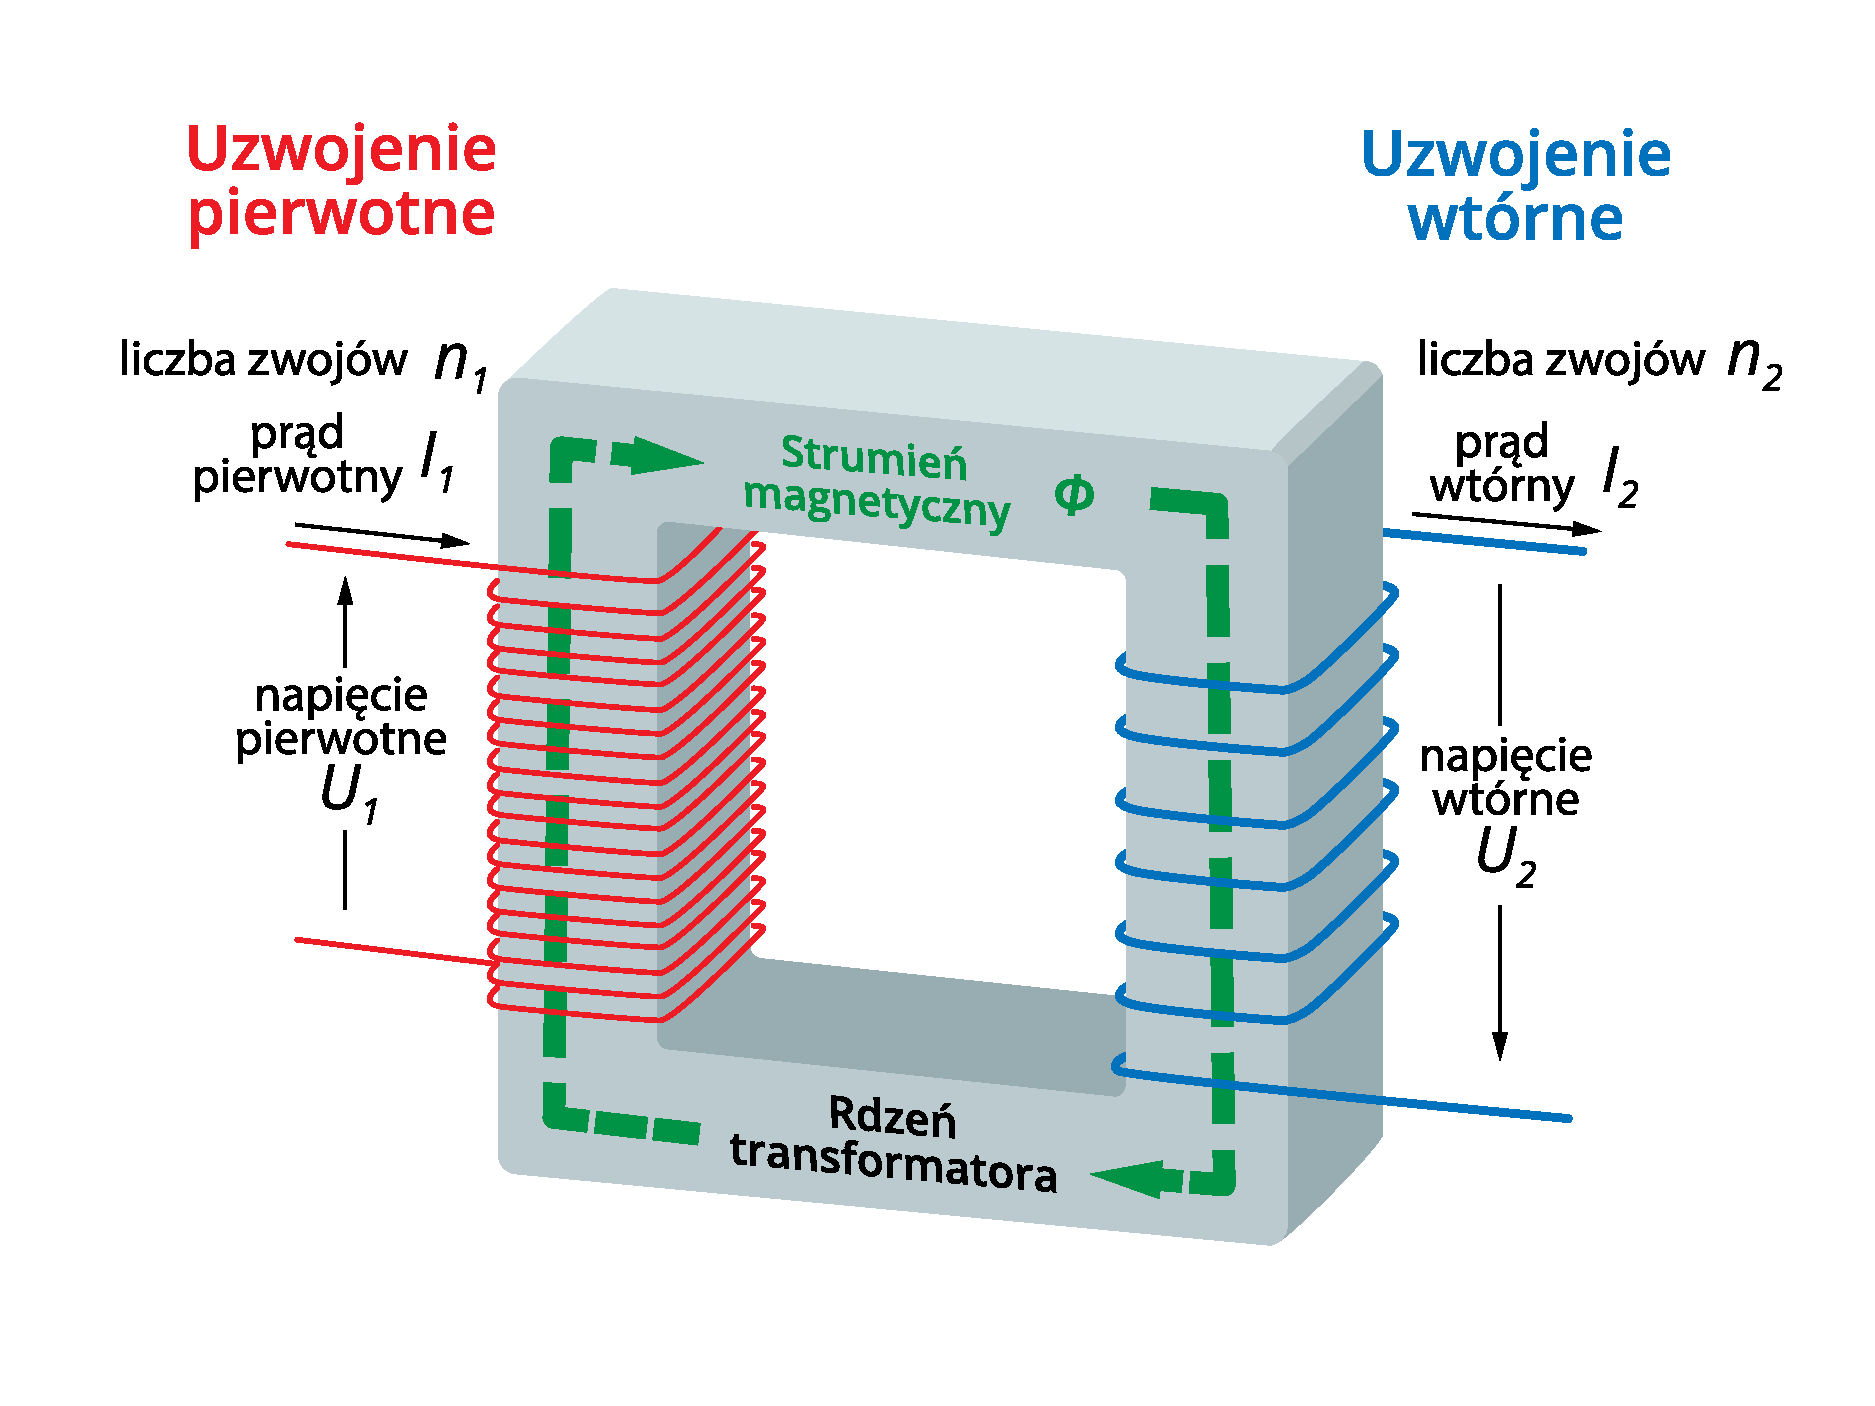
\includegraphics[width=0.6\textwidth]{transf.pdf}

  \columnbreak
  
  \centering
  $$\frac{U_2}{U_1} = \frac{n_2}{n_1}$$\\ \vspace{0.15cm}
  
  Moc wejsciowa jest równa wyjściowej: $P_1 = P_2$
\end{multicols}

Moc i praca prądu:\\
$P = U\cdot I$\\ 
$W = U\cdot I\cdot t$


\end{tcolorbox}

% TERMODYNAMIKA
\begin{tcolorbox}[title=\textbf{Termodynamika}, colframe=pastelgreen, colback=white]
Pierwsza zasada termodynamiki: \\
$\Delta U = Q - W$\\[6pt]
Równanie Clapeyrona: \\
$pV = nRT$
\end{tcolorbox}

% OPTYKA
\begin{tcolorbox}[title=\textbf{Optyka}, colframe=pastelviolet, colback=white]

\begin{multicols}{2}

Równanie soczewki: \\
$\frac{1}{f} = \frac{1}{d_o} + \frac{1}{d_i}$\\[6pt]
Wzór na powiększenie: \\
$M = \frac{h_i}{h_o} = -\frac{d_i}{d_o}$

\end{multicols}
% Rysunek soczewki

% Ulepszony rysunek soczewki

\begin{center}
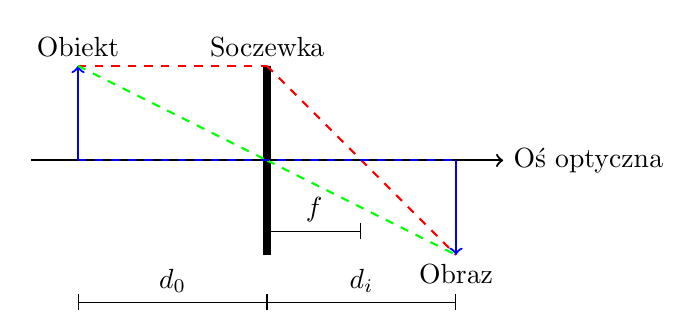
\begin{tikzpicture}[scale=0.6]
    % Oś optyczna
    \draw[thick,->] (-5,0) -- (5,0) node[right] {Oś optyczna};
    
    % Soczewka
    \draw[line width=1mm] (0,-2) -- (0,2);
    \node[above] at (0,2) {Soczewka};
    
    % Obiekt
    \draw[thick,->,blue] (-4,0) -- (-4,2);
    \node[above] at (-4,2) {Obiekt};
    
    % Promienie świetlne
    \draw[thick,red,dashed] (-4,2) -- (0,2);
    \draw[thick,red,dashed] (0,2) -- (4,-2);
    
    \draw[thick,green,dashed] (-4,2) -- (0,0);
    \draw[thick,green,dashed] (0,0) -- (4,-2);
    
     \draw[thick,blue,dashed] (-4,0) -- (4,0);
   
    % Obraz
    \draw[thick,blue,->] (4,0) -- (4,-2);
    \node[below] at (4,-2) {Obraz};

    \def\vary{-3}  % Defines \varx as 3 (doesn't evaluate math)

    \node[above] at (-2,\vary) {$d_0$};
    \node[above] at (2,\vary) {$d_i$};

     \draw[|-|] (0,\vary) -- (4,\vary);
     \draw[|-|] (-4,\vary) -- (0,\vary);

     \node[above] at (1,\vary/2) {$f$};
     \draw[|-|] (0,\vary/2) -- (2,\vary/2);
    

\end{tikzpicture}
\end{center}


\end{tcolorbox}

\begin{tcolorbox}[title=\textbf{Kinematyka}, colframe=pastelorange, colback=white]
$$v = \frac{\Delta x}{\Delta t}$$\\
$$a = \frac{\Delta v}{\Delta t}$$
\end{tcolorbox}


\end{multicols}



\end{document}
